\documentclass[10pt,a4paper]{article}
\usepackage[utf8]{inputenc}
\usepackage{amsmath}
\usepackage{amsfonts}
\usepackage{amssymb}
\usepackage{graphicx}
\author{Rafael Perazzo Barbosa Mota}
\title{Q Algorithm}
\begin{document}
\maketitle

\section{Q Algorithm Fluxogram}

\begin{figure}[!htb]
\centering
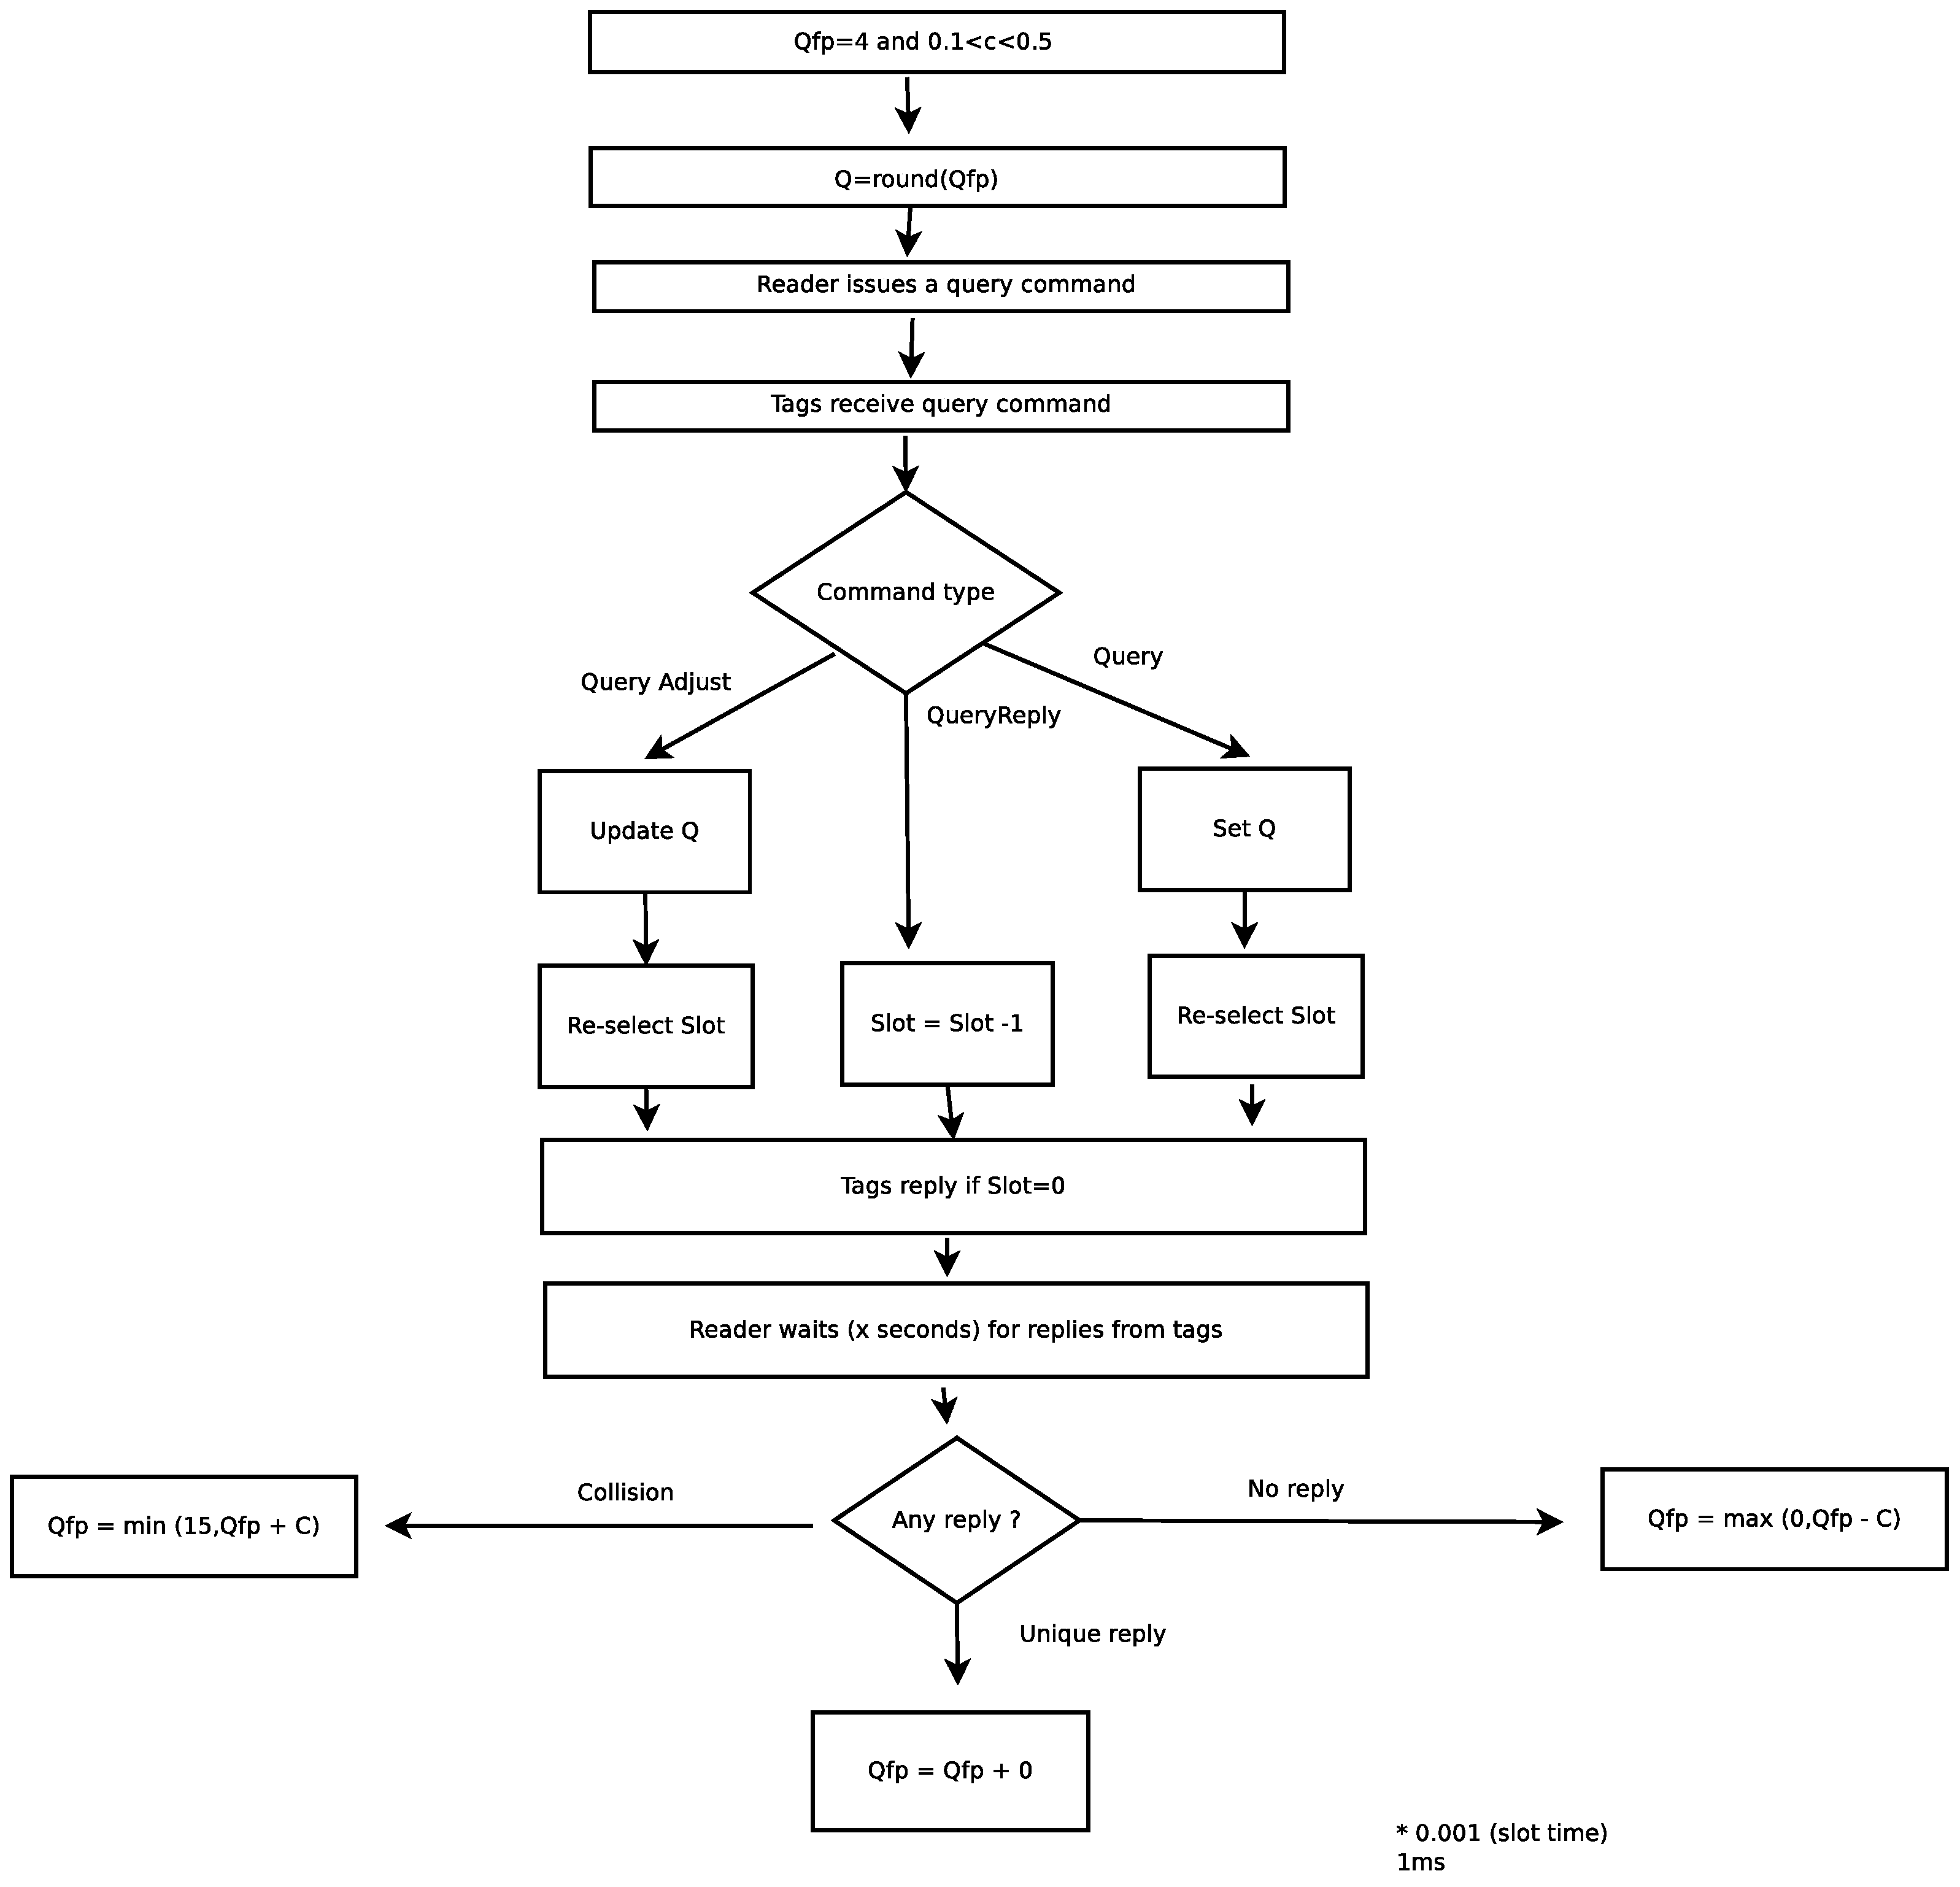
\includegraphics[scale=0.25]{imagens/QAlgorithm.eps}
\caption{ {\small Q Algorithm Fluxogram}}
\label{fig:1}
\end{figure}	

\section{Tags states diagram}

\begin{figure}[!htb]
\centering
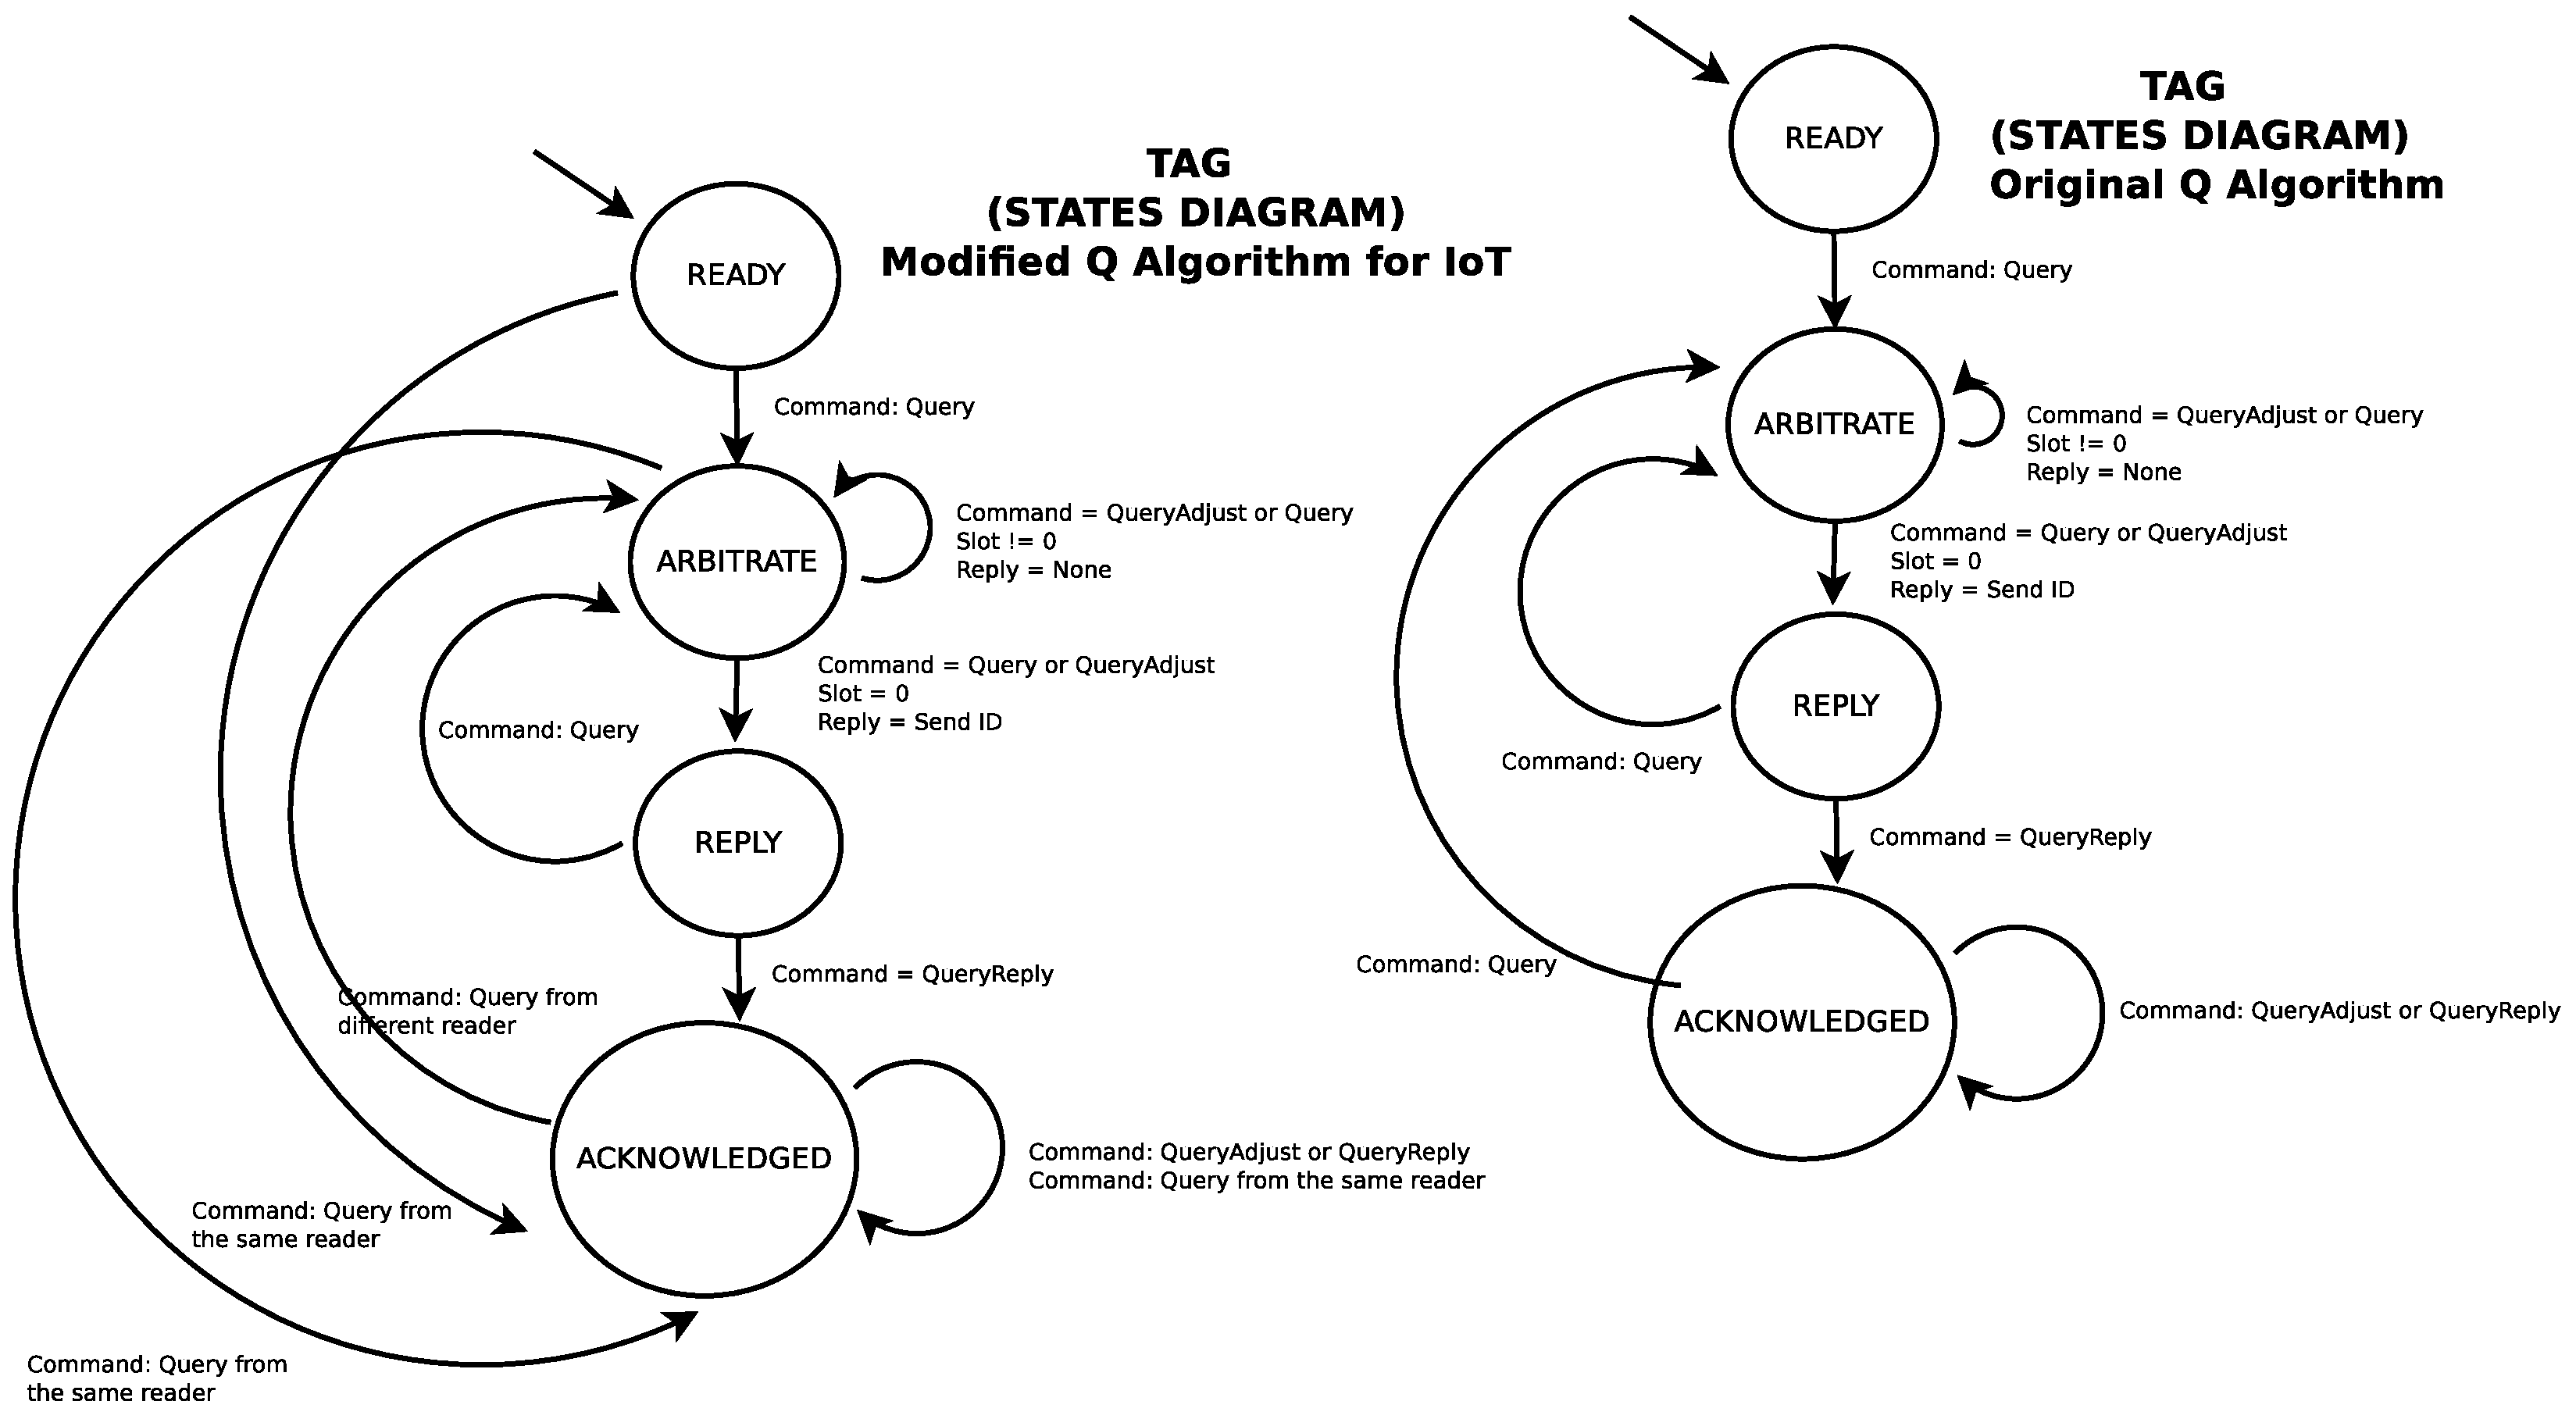
\includegraphics[scale=0.25]{imagens/QAlgorithm_StateDiagram.eps}
\caption{ {\small Q Algorithm tags state machine (Original and Modified)}}
\label{fig:2}
\end{figure}	

\section{Number of tags identified per time}

\begin{figure}[!htb]
\centering
\includegraphics[scale=0.9]{imagens/identification.eps}
\caption{ {\small Performance analysis of Q Algorithm simulation}}
\label{fig:3}
\end{figure}	

\section{Inventory application scenario}

	Supply Chain Management (SCM) is the ``management and control of all materials and information in the logistics process from acquisition of raw materials to delivery to the end user'' \cite{r1}. Smart shelves have been studied by several research groups, and  a number  of  industrial initiatives already apply these technologies \cite{r2,r3,r4}.

\begin{figure}[!htb]
\centering
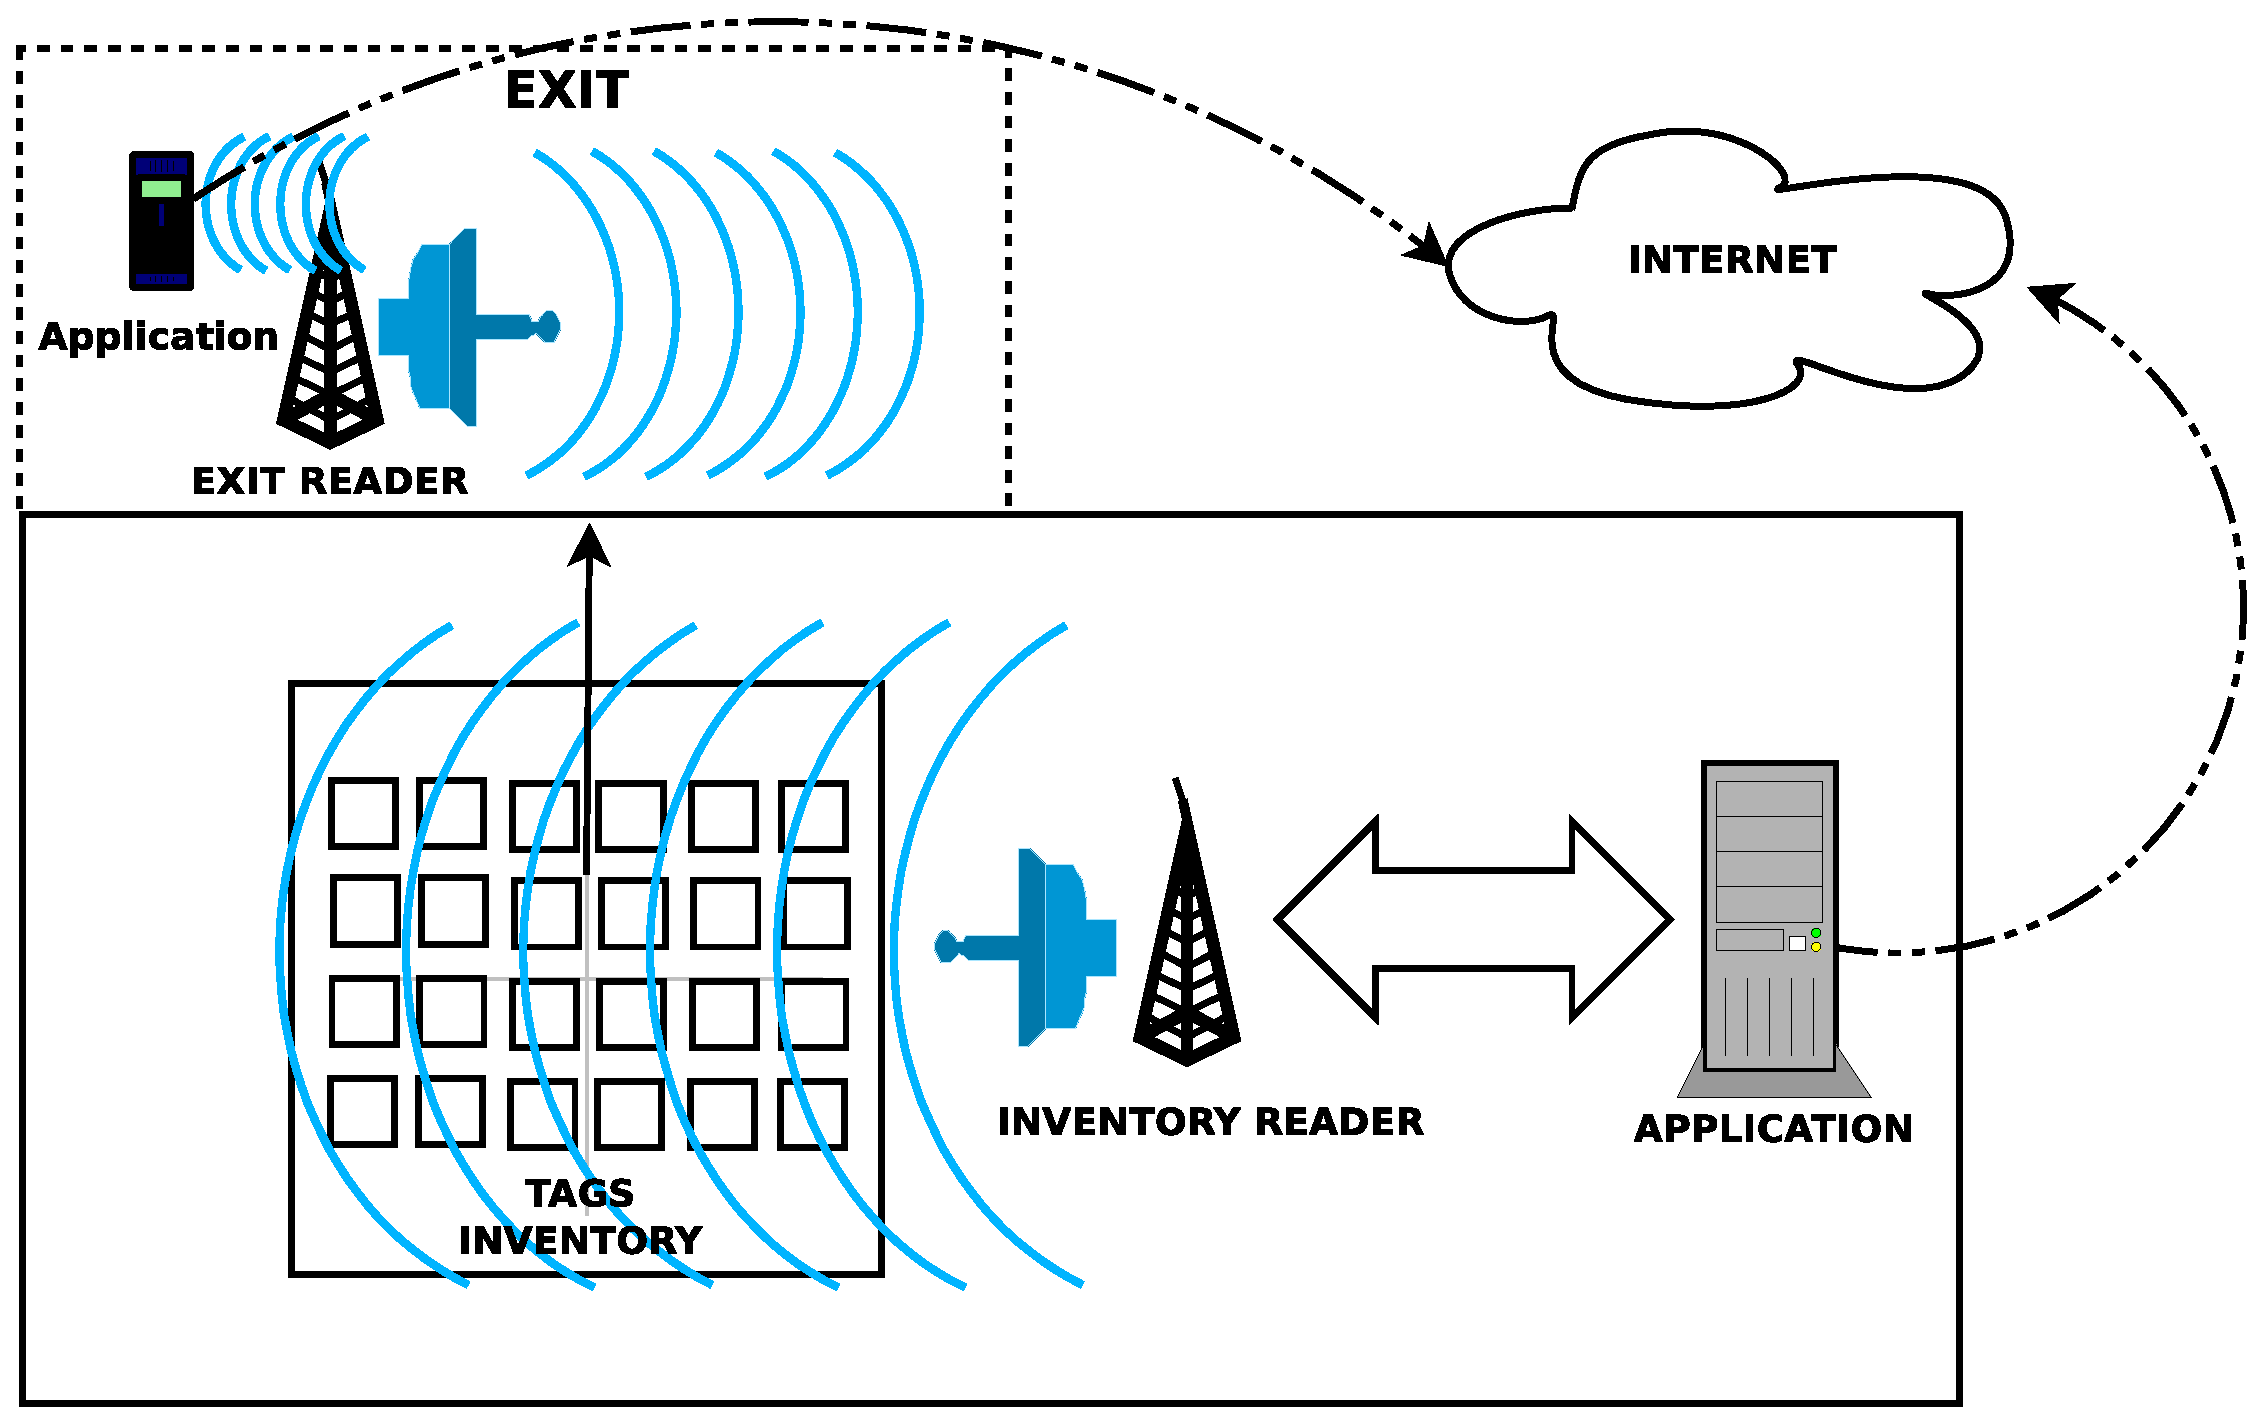
\includegraphics[scale=0.4]{imagens/cenario.eps}
\caption{ {\small Example of Inventory IoT application}}
\label{fig:4}
\end{figure}	

\begin{thebibliography}{9}

\bibitem{r1}
  Michael, K.; McCathie, L.; , ``The pros and cons of RFID in supply chain management,'' Mobile Business, 2005. ICMB 2005. International Conference on , vol., no., pp. 623- 629, 11-13 July 2005
doi: 10.1109/ICMB.2005.103

\bibitem{r2}

Hinske, Steve; , ``Determining the Position and Orientation of Multi-Tagged Objects Using RFID Technology,'' Pervasive Computing and Communications Workshops, 2007. PerCom Workshops '07. Fifth Annual IEEE International Conference on , vol., no., pp.377-381, 19-23 March 2007
doi: 10.1109/PERCOMW.2007.38

\bibitem{r3}

Aysegul Sarac, Nabil Absi, and Stéphane Dauzère-Pérès. 2008. A simulation approach to evaluate the impact of introducing RFID technologies in a three-level supply chain. In Proceedings of the 40th Conference on Winter Simulation (WSC '08), Scott Mason, Ray Hill, Lars Mönch, and Oliver Rose (Eds.). Winter Simulation Conference 2741-2749.

\bibitem{r4}

Blau, J.; , ``Supermarket's futuristic outlet'', Spectrum, IEEE , vol.41, no.4, pp. 21- 22, 25, April 2004
doi: 10.1109/MSPEC.2004.1279188

\end{thebibliography}

\end{document}